The Getting Started section explains how to create a new project based on the \texttt{refman} template, then use Overleaf's interface to configure the project. Before starting, ensure you have an Overleaf account by registering at \url{https://www.overleaf.com/register}.

\begin{minipage}{\linewidth}
\fbox{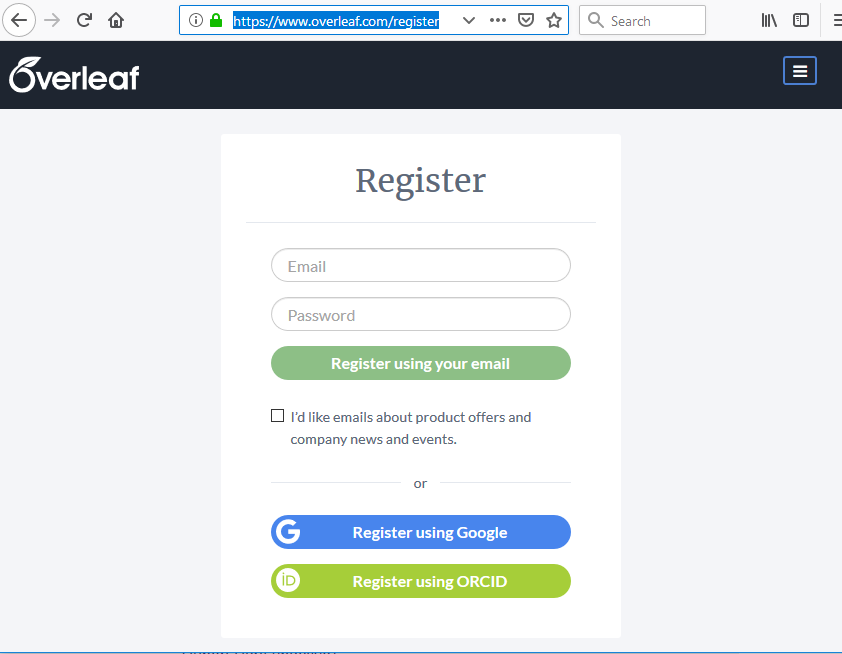
\includegraphics[width=\linewidth]{graphics/RegisterOverleaf.PNG}}
\captionof{figure}{Overleaf registration site \texttt{refman}}
\end{minipage}

\subsection{Requirements Setup}


\subsection{Creating Project}

\subsection{Main Screen}

\subsection{Configuring Project}

